% !TeX root = ../main.tex

\chapter{需求分析}

\section{系统概述}
容器化 CI/CD 流水线调度系统是一个自动化的工具,旨在提高软件开发的效率和速度。
它通过自动化编译、测试和部署过程,实现持续集成和持续交付。
该系统将支持敏捷开发的实践,通过自动化任务调度来优化研发团队的工作流程。
\section{需求导出}

首先,我们要明确我们的目标是设计一个高效、灵活且可靠的容器化CI/CD流水线调度系统。
该系统不仅要能够让用户根据自己的需求高度定制化自己的流水线,并提供稳定的执行,而且还要确保这一过程尽可能自动化,减少手动干预,提高开发效率和代码质量。
此外,系统还需要能够适应不断变化的开发需求,支持快速迭代,以满足敏捷开发的要求。

在了解这些基本目标之后,本文通过与企业内各个利益相关者的深入访谈,识别出了以下具体需求:

\subsubsection{开发团队需求}
开发团队期望系统能提供一站式服务,自动完成从代码提交到部署的整个流程。
并且对系统的定制性有一定要求,开发团队希望流水线系统支持丰富的功能支持,以便满足多样化的需求。
同时开发人员希望流水线以及流水线中作业、任务能够最好以模板化、插件化的形式存在,以便开发人员能够以最高的效率完成流水线的定义与配置,从而将更多精力投入到开发工作本身。

\subsubsection{测试团队需求}
测试团队希望流水线平台能够充分自动化,以缓解测试的人力资源需求,希望系统能够自动执行各种测试,包括单元测试、集成测试和性能测试等;
同时希望系统能够生成详细的测试报告,帮助测试人员快速发现和跟踪问题。

\subsubsection{运维团队需求}
运维团队更加注重功能性和稳定性。运维团队希望系统支持庞大而复杂的流水线,以支持企业软件栈全面的集成与交付。
同时希望流水线能够支持一系列的人工操作,以便在流水线的执行过程中对流水线进行干预和把控。
稳定性方面,由于企业内存在周期性的发布高峰,运维团队希望系统能够应对高峰期时的突发流量,并且出现异常时能快速恢复,以保证高可用性。

结合以上需求,我们希望能够设计出一个不仅功能强大,而且可用性强、稳定可靠的CI/CD流水线调度系统。

\section{功能性需求}

\subsection{术语描述}
为了清晰地描述系统需求,首先需要对CI/CD流水线中一些基本术语进行解释:

\subsubsection{任务(Task)}
任务表示流水线中执行的一个单独的、不可再分的原子任务。
一个原子任务只完成一件事,如拉取Gitlab仓库代码、开源合规扫描、执行一个Shell脚本等。
任务必须包含在作业(Job) 内,同一个作业内的任务按顺序串行执行。

\subsubsection{作业(Job)}
作业表示流水线中将要调度到执行器中执行的一系列原子任务的集合,是执行器执行的最小单位。
一个作业将运行在一个独立的运行环境中,它有以下特性:
\subparagraph{由多个任务组成;}
\subparagraph{作业内一个任务失败,则整个作业失败,其余任务将不会运行。}

\subsubsection{阶段(Stage)}
阶段是一系列作业的逻辑集合。它的存在是为了更清晰的描述和管理流水线,它有以下特性:
\subparagraph{由多个作业组成;}
\subparagraph{同一个阶段下的不同作业执行方式为并行,当某个作业失败后,其它的作业会继续运行;}
\subparagraph{阶段内一个作业失败,则整个阶段失败。}

\subsubsection{流水线(Pipeline)}
流水线是一个执行一系列作业的自动化工作流,它有以下特性:
\subparagraph{由多个阶段组成;}
\subparagraph{同一个流水线下的阶段串行执行,一个阶段失败,将不会执行后续阶段;}
\subparagraph{流水线内一个阶段失败,则该流水线失败。}

图~\ref{fig:流水线示意图}是图~\ref{fig:典型流水线示意图}的流水线按照以上概念进行的逻辑边界划分,它反映了流水线、流水线阶段、流水线作业和流水线任务的层级关系。
当该流水线被手动触发后则进入第一个阶段,该阶段包括两个作业——单元测试和静态代码检查,这两个作业将并行执行,在作业执行的过程中,每个作业内部的任务将顺序执行。
当这两个作业都成功后,流水线进入第二个阶段,再执行第二个阶段中的作业——编译并上传镜像。
以此类推,在没有人工干预的情况下,流水线将自动化地执行下去,直到某个作业执行失败则流水线失败,所有作业都执行成功则流水线成功。

\begin{figure}[h]
  \centering
  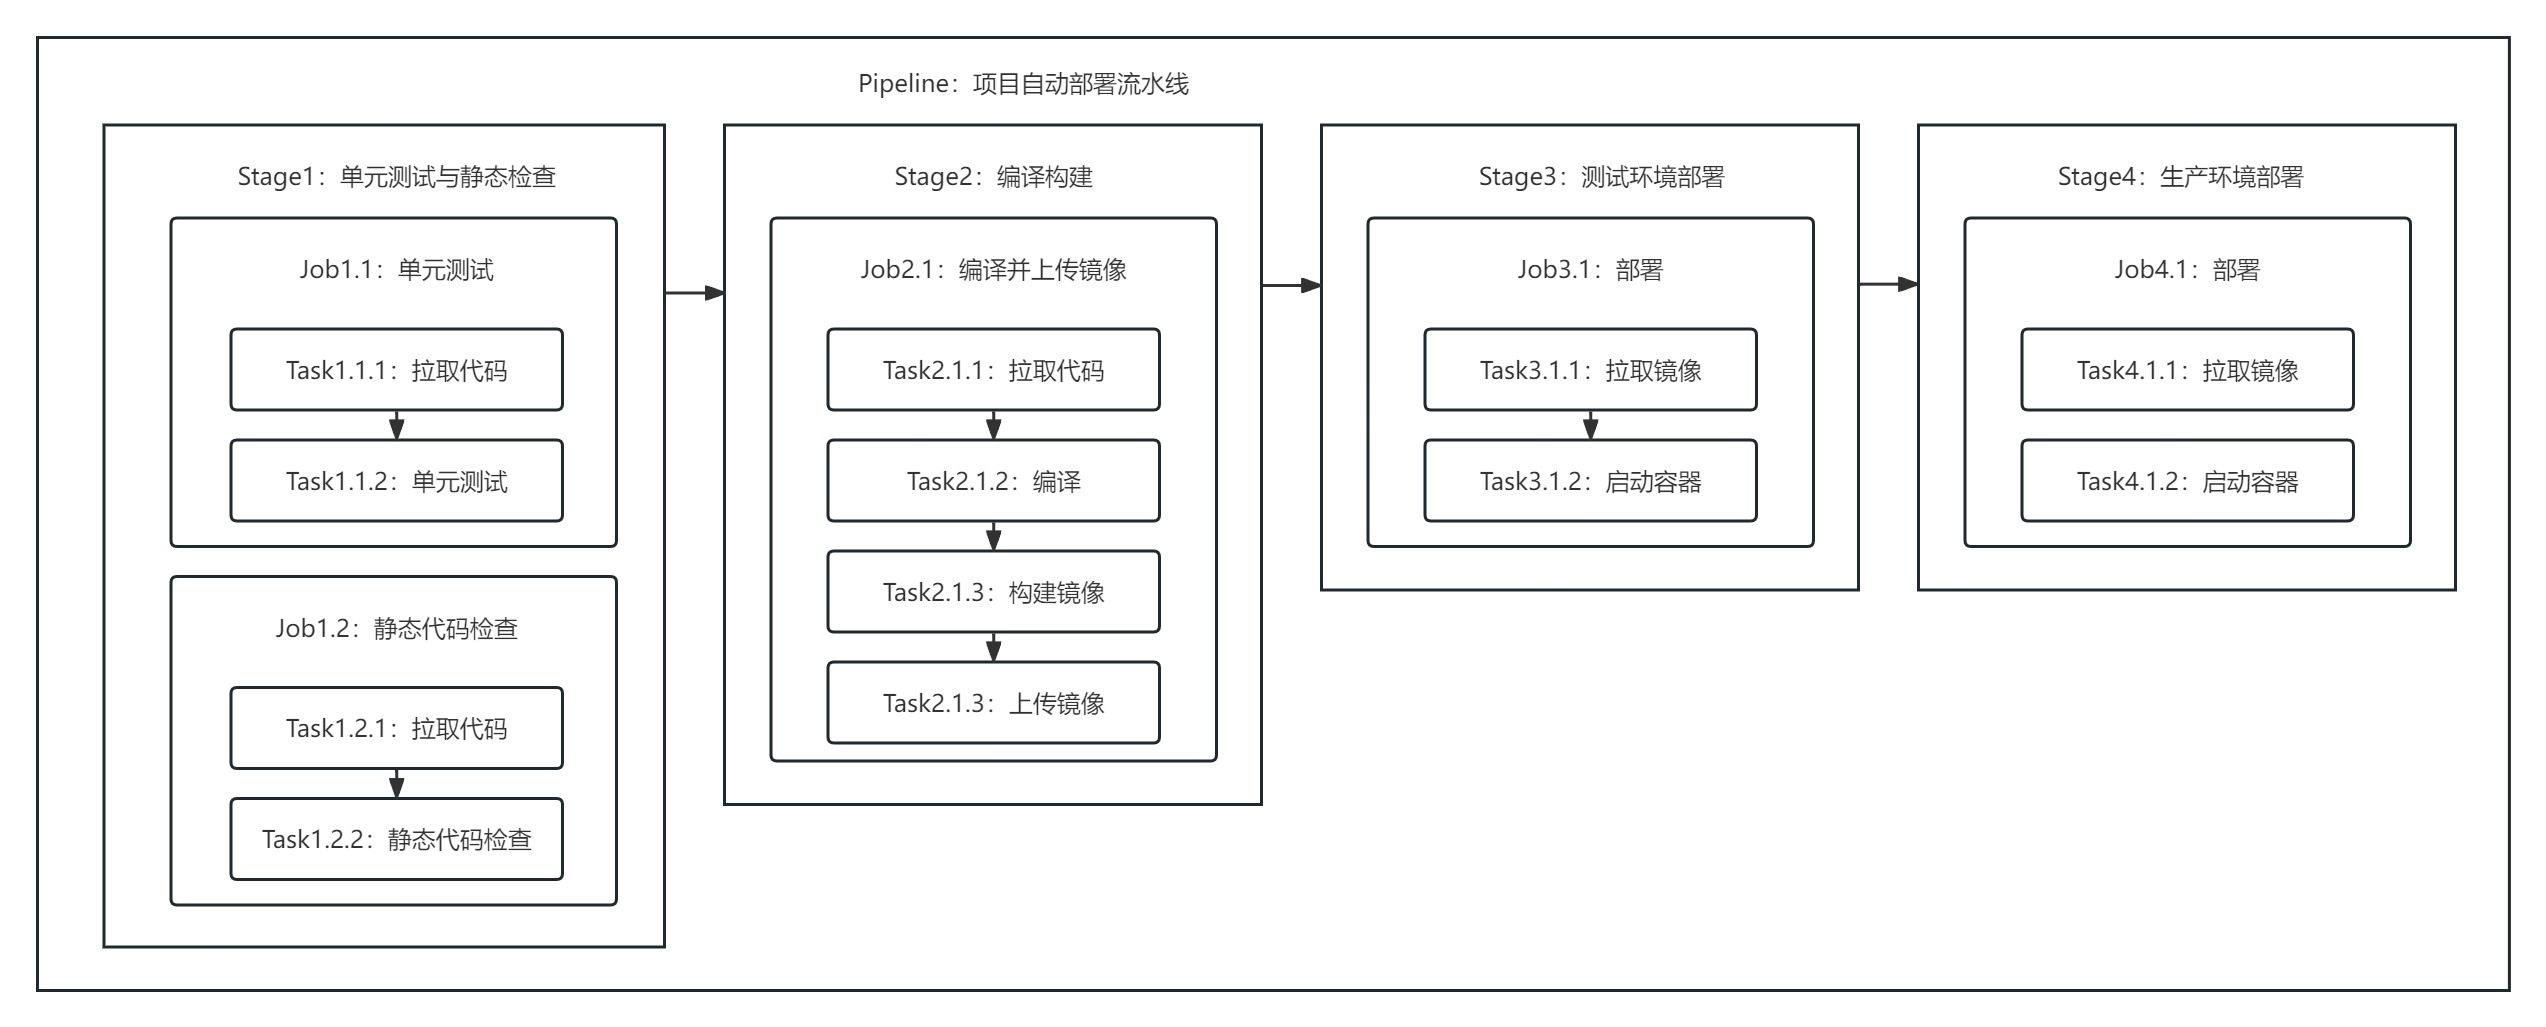
\includegraphics[width=1\textwidth]{流水线示意图.jpg}
  \caption{流水线示意图}
  \label{fig:流水线示意图}
\end{figure}

\subsection{流水线管理需求}
对于一个流水线系统来说,需要提供给用户对流水线进行增删改查的基本操作,主要包括:

\subsubsection{创建并配置流水线}
CI/CD流水线的形态十分复杂,包含了三种不同类型的子概念:阶段、作业和任务,每个子概念中又有一系列的属性需要配置,如名称、触发类型等。
创建流水线时仅仅只创建流水线是无法运行的,流水线本质上只是对流程的抽象,对其中子概念的封装,所以创建流水线的同时必须同时进行一系列配置。

在创建流水线时,用户首先需要根据其业务需求,创建出不同的子概念,比如用户想要创建一个支持编译、测试和部署的流水线,用户则可以先按顺序创建出三个流水线阶段,
再在界面中通过拖拽等方式编排各个阶段的位置,以体现不同阶段的前后顺序,再在不同的阶段里创建一系列的作业,最后在已创建的作业里创建任务,至此完成了流水线结构的创建;
然后,用户需要进行流水线配置,也就是规定流水线中各个作业和任务都要做什么事情,系统应为每个用户已创建的子概念提供表单,以便用户为各个子概念填写配置信息。

总而言之,创建流水线时,系统需要提供给用户友好的交互页面,以便用户完成流水线结构的创建与配置填写。

\subsubsection{编辑流水线配置}

系统应支持用户编辑已创建好的流水线,方便用户根据业务需求对流水线的结构和配置进行调整。

\subsubsection{查看流水线配置及其运行记录}
系统提供友好的UI界面以便用户查看流水线配置。
同时,因为一条流水线能够被反复运行,所以一条流水线会产生多次运行记录,包括当次运行的各个子概念的最终状态、运行时间、日志等等,这些运行记录也应提供入口给用户查看。

\subsubsection{删除流水线}
系统应支持用户删除不再使用的流水线。

流水线管理模块用例图如图~\ref{fig:流水线管理用例图}所示。

\begin{figure}[h]
  \centering
  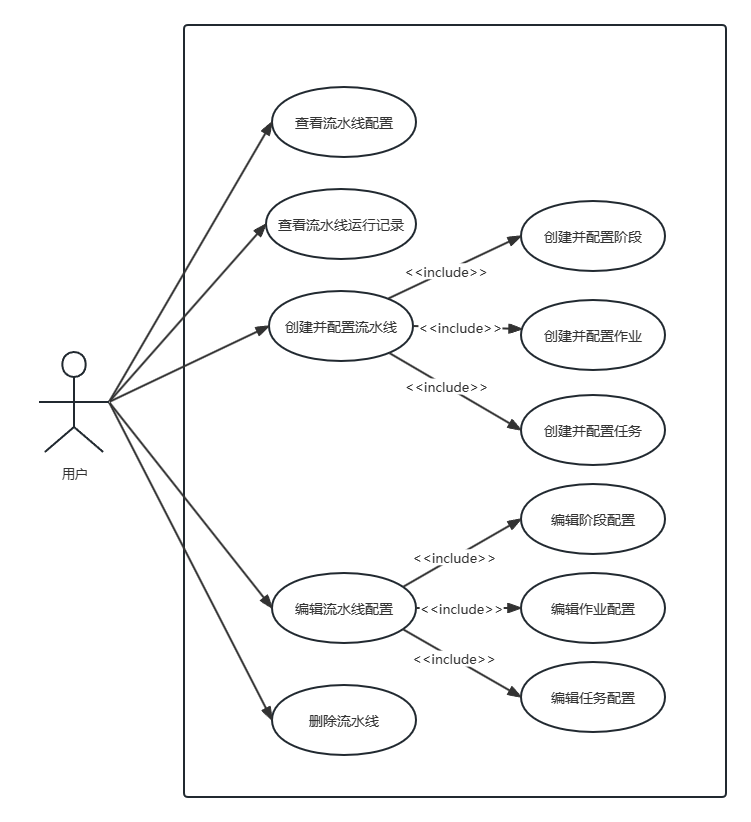
\includegraphics[width=0.7\textwidth]{流水线管理用例图.png}
  \caption{流水线管理用例图}
  \label{fig:流水线管理用例图}
\end{figure}

\subsection{人为干预流水线需求}
当用户使用已经创建好的流水线的过程中,为满足用户对流水线的复杂操作需求,提高流水线的灵活度,CI/CD调度系统需要支持用户在流水线执行过程中主动对流水线的执行情况进行干预;
干预行为主要包括:

\subsubsection{手动触发(Trigger)}
流水线的触发通常分为自动触发和手动触发两种方式

\subsubsection{取消(Cancel)}
当用户在流水线的运行过程中,意识到流水线的后续执行会产生自己不期望的后果时,CI/CD调度系统应支持用户将其取消。
注意,当阶段或作业被取消后,系统应视为其已经失败,应阻止与其串行的后续阶段或作业的继续执行。

\subsubsection{重试(Retry)}
流水线中某个作业的失败往往不是必现的,当用户认为某个失败的作业并非源于配置或者代码本身,而是因为运行环境、网络稳定性等因素导致失败时,CI/CD调度系统应支持用户将其重试。

\subsubsection{跳过(Skip)}
通常来说,一条精心配置的流水线包含非常多的阶段和作业。但复用这条流水线的各个用户的需求可能各不相同。
当某个阶段或者作业用户认为没有必要执行,或者运行时间过长用户不希望再等待时,CI/CD调度系统应支持用户将其跳过。
注意,与“取消”操作相反,当阶段或作业被跳过后,系统应视为其已经成功,应立即继续与其串行的后续阶段或作业的继续执行。

\subsubsection{人工审核(Review)}
当流水线运行到某个阶段或某个作业时,为确保后续按期望执行,并保证流水线产物的质量,CI/CD调度系统应支持用户在某个阶段或作业开始前,加入人工审核的环节。
同时,这一功能应支持流水线的编辑者自行设置审核人和审核的通过条件,比如设置了两位部门领导作为审核人,当任意一位审核人进入系统并点击“准入”后,该阶段或作业即开始执行;当两位审核人都点击“中止”后,该阶段或作业则被视为取消。

以上人工干预行为分别适用于一个或多个流水线中的子概念(流水线、阶段、作业和任务),依据对常见业务场景的分析,各个概念应支持的人工干预行为如表~\ref{tab:各个子概念应支持的人为干预行为表}:
\begin{table}[h]
  \centering
  \caption{各个子概念应支持的人为干预行为表}
  \label{tab:各个子概念应支持的人为干预行为表}
  \begin{tabular}{cl}
    \toprule
    子概念     & 人为干预行为                                     \\ 
    \midrule
    流水线     & 手动触发、取消 \\
    阶段       & 人工审核、取消、重试、仅重试阶段中失败作业   \\
    作业       & 手动触发、人工审核、取消、跳过、重试      \\
    任务       & 不允许人为干预       \\
    \bottomrule
  \end{tabular}
\end{table}

综上,得出流水线人为干预模块用例图如图~\ref{fig:流水线人工干预用例图}所示。

\begin{figure}[h]
  \centering
  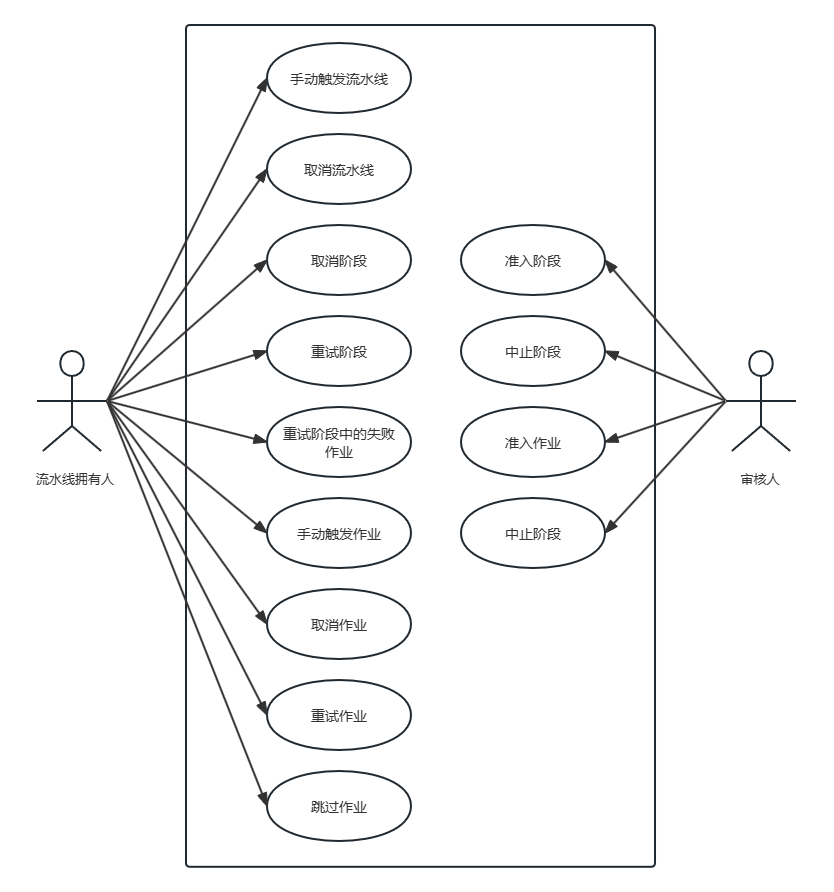
\includegraphics[width=0.8\textwidth]{流水线人工干预用例图.png}
  \caption{流水线人工干预用例图}
  \label{fig:流水线人工干预用例图}
\end{figure}

\subsection{节点管理需求}
流水线作业最终会被具象为一段脚本或者可执行文件,“节点”则是这个脚本或可执行文件的实际运行环境,
这个环境可以是物理服务器、虚拟机或者容器。
系统应允许用户主动对节点进行配置和部署,有以下几点原因:
\begin{enumerate}
  \item 适应不同作业需求。不同的作业需要的资源配置可能会有较大差异,比如AI的训练与推理对实际运行环境的算力资源有需求,
  用户则需要自己提供并指定一台带有对应硬件设备的服务器,并在系统中注册为节点以保证AI的训练与推理作业能够顺利完成。
  允许用户自定义节点能够确保每个项目能够在最适合其需求的环境中运行,从而提高构建和部署的效率。
  \item 环境隔离。并不是所有的作业都适合在虚拟机或者容器化的环境中运行,在某些场景下,特定的任务可能需要在隔离的物理机环境中运行以满足安全性要求。
  用户自定义节点允许为这些任务创建特定的安全配置和隔离环境。
  \item 提高灵活性和可扩展性。自定义的节点可以保证系统能够适应快速变化的技术和业务需求,支持新技术的快速集成和应用。
\end{enumerate}

用户对节点的管理主要包括如下内容:
\subsubsection{注册节点}
节点注册是将新节点引入系统的过程,系统为用户提供预设的配置模板,用户填写对应节点的IP、端口、标签(Tag)、环境变量、部署类型等选项后,该节点将被注册到系统中,供后续部署上线。

\subsubsection{一键部署}
为了充分降低用户使用成本,系统应提供节点的一键部署功能。
用户可以一键将系统的执行器远程部署到目标服务器,并自动完成与本系统的对接。
这项功能减少了配置新节点所需的手动操作,提高了部署效率,大幅提高系统的可用性。

\subsubsection{节点上下线}
此功能允许节点根据系统负载和维护计划自动或手动地切换其活动状态。上线的节点准备接受新任务,而下线的节点则不再分配新任务,已有任务继续执行至完成。
这样的机制确保了系统能够在不同的运行条件下维持最优的资源利用和稳定性。

\subsubsection{删除节点}
删除节点功能使得管理员能够从系统中移除不再需要或过时的节点,包括清理与这些节点相关的配置信息和数据。这不仅有助于资源的合理管理,也保持了系统的整洁性和高效运行。

节点管理的用例图如图~ \ref{fig:节点管理用例图}所示。
\begin{figure}[h]
  \centering
  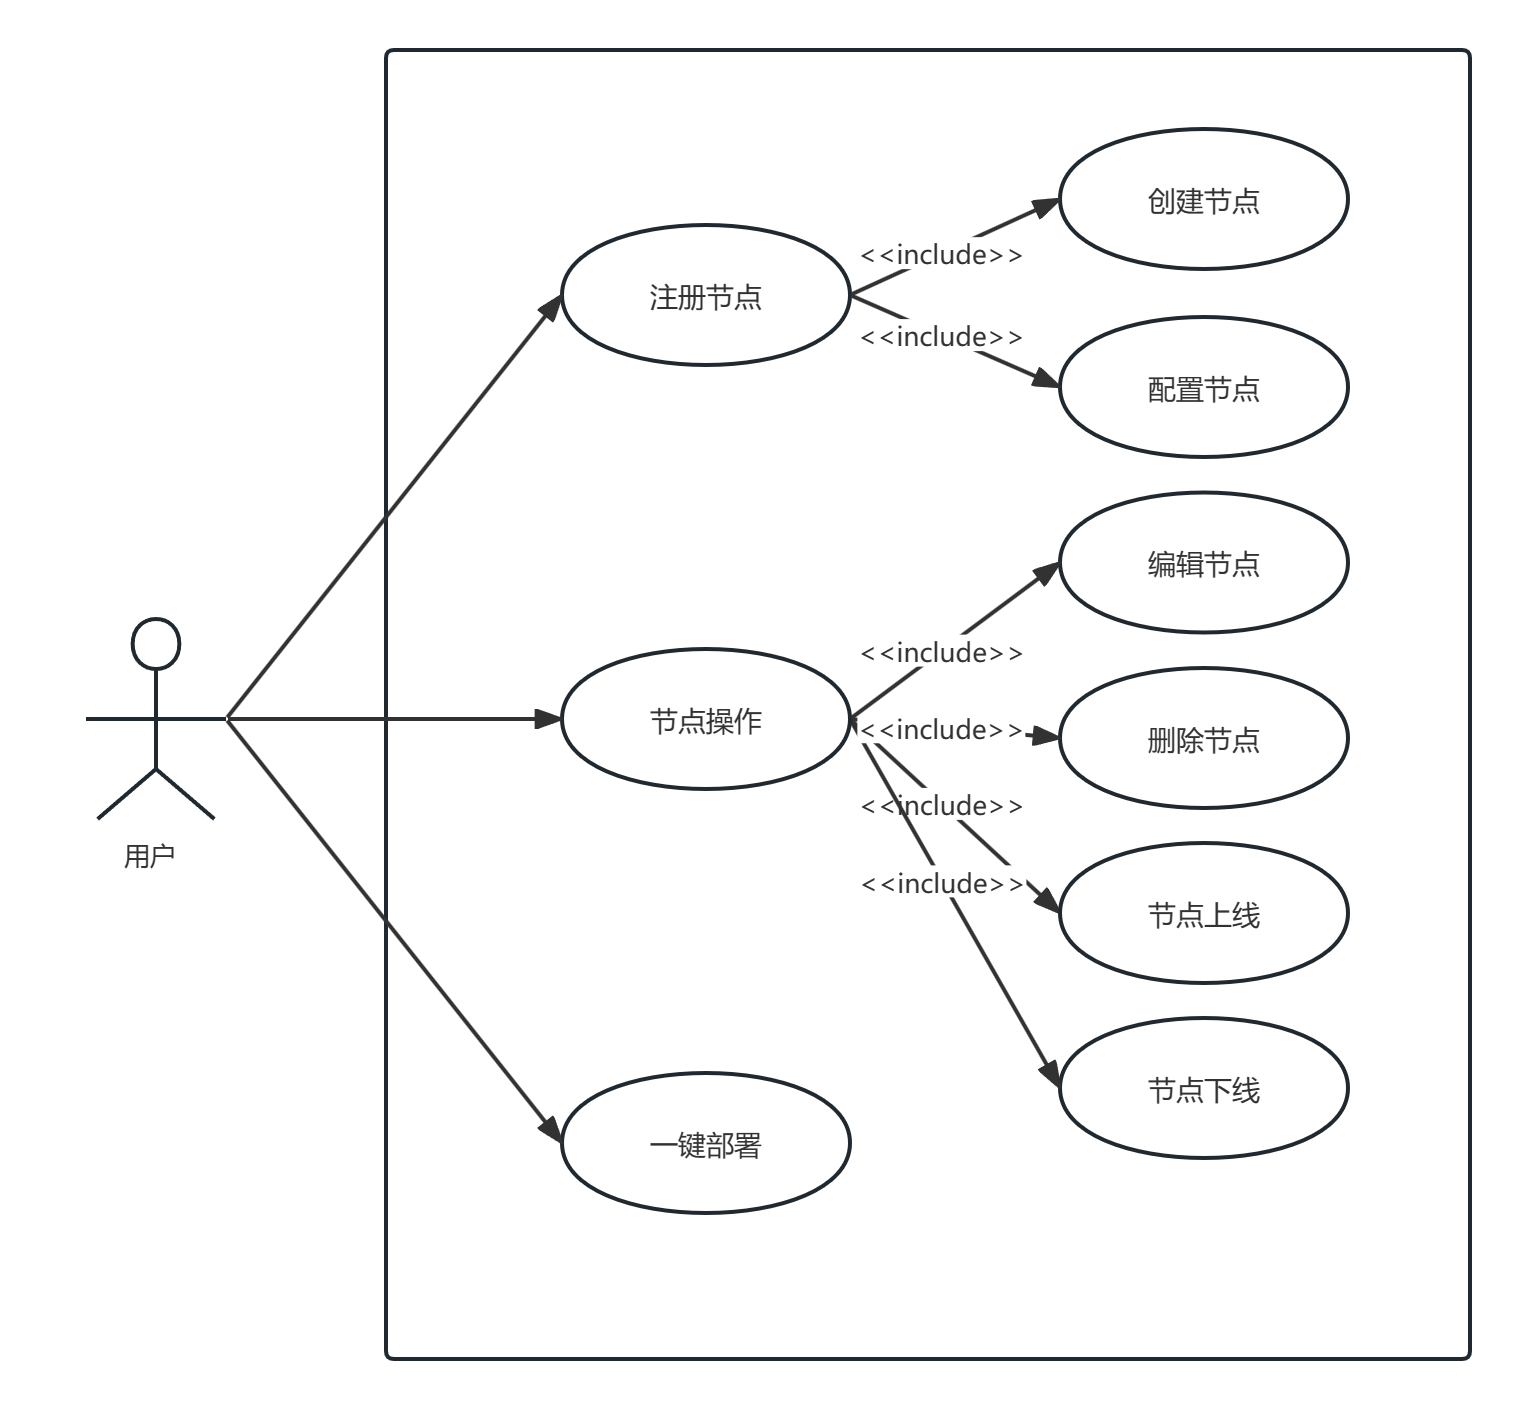
\includegraphics[width=0.7\textwidth]{节点管理用例图.png}
  \caption{节点管理用例图}
  \label{fig:节点管理用例图}
\end{figure}

\subsection{Docker镜像管理需求}
在CI/CD流水线系统中,绝大多数流水线运行的作业都是通过Docker容器进行的,这直接要求系统必须提供多样化的Docker镜像以供用户选择,以满足不同作业的运行需求。
镜像管理因此成为系统执行多样化的作业的重要前置功能,负责镜像的制作、上传、删除和详情查看等功能。
有效的镜像管理不仅保障了容器化作业的顺利执行,也提高了整个系统的灵活性和可用性。

用户对Docker镜像的管理主要包含以下内容:

\subsubsection{镜像制作}
镜像制作的自动化和安全化是镜像管理的核心。本系统应提供两种制作镜像的方法:

一是通过DockerFile构建,这种方式为高度自动化和定制化的镜像制作提供了可能,用户通过编写DockerFile来定义镜像的构建过程。这要求用户对DockerFile的语法和构建过程有深入理解。
二是使用commit提交,这种方式适用于需要手动环境配置的场景,通过将运行中的容器状态提交为新的镜像。这种方法依赖于SSH协议远程连接容器,保障了操作的安全性。

\subsubsection{镜像删除}
考虑到存储资源的有效利用,镜像删除功能是镜像管理不可或缺的一部分。本系统通过引入引用计数机制,确保不再被需要的镜像能够被有效清理,释放存储空间,同时解决了传统删除机制无法彻底删除底层文件的问题。

\subsubsection{镜像上传}
镜像上传过程中维护Layer引用记录文件的完整性和准确性是镜像管理的另一关键点。这一机制确保了镜像仓库的数据一致性和完整性,特别是在镜像频繁更新的环境下尤为重要。

镜像管理的用例图如图~ \ref{fig:镜像管理用例图}所示。

\begin{figure}[h]
  \centering
  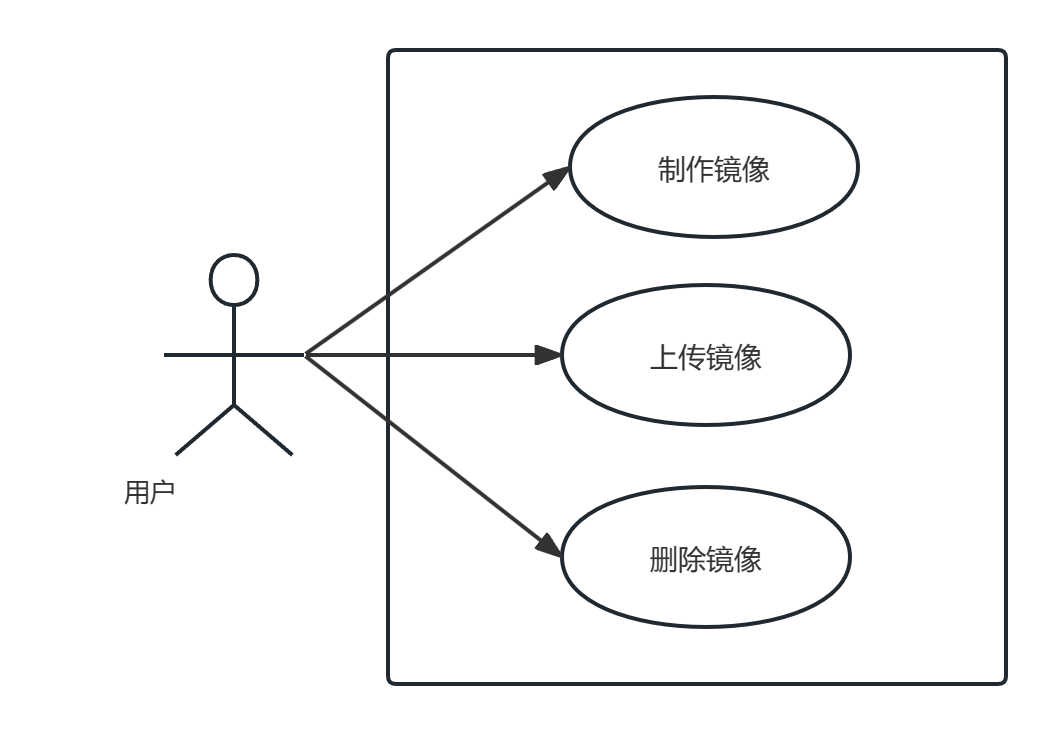
\includegraphics[width=0.7\textwidth]{镜像管理用例图.png}
  \caption{镜像管理用例图}
  \label{fig:镜像管理用例图}
\end{figure}

\subsection{插件化需求}
CI/CD流水线系统的最终目的是提高企业用户的开发效率。
市面上现有的持续集成系统,在用户配置流水线的作业时,往往只有系统预置的一些功能模块可供选择,大大限制了系统的灵活性;
又或是需要用户亲自进行大量的配置和脚本编写,以满足一条复杂流水线中不同作业的需求。
为处理这种灵活性与效率之间的矛盾,插件化是一种很好解决方式,系统管理团队将会预提供一个丰富多样的插件库,同时也需支持用户自行定义插件,自用或发布到插件市场中。
如此一来,当用户构建一条流水线时,可以根据自己选择不同的插件来组合成流水线作业,从而快速完成流水线的配置。

插件市场中主要包含如下内容:

\subsubsection{插件管理}
在CI/CD系统中,插件本质上是对一套配置清单和一个执行脚本的抽象,这种设计旨在简化插件的使用和集成过程,使用户能够通过填写配置清单来定制插件行为,然后执行脚本以在CI/CD流程中实现特定功能。
系统应让用户能够轻松管理和编写自己的自定义插件,同时提供一种机制,使用户能够编辑出属于该插件的配置清单(即使用该插件时需要填写的配置信息),并确保脚本的安全、有效执行。
同时,系统应支持插件的版本管理。每当插件更新时,应记录版本历史,允许用户选择特定版本进行安装。如果新版本存在问题,这一机制确保了用户可以轻松回退到旧版本。

\subsubsection{插件发布}
开发者在自定义插件并满足个人或团队需求后,可以选择将其发布到插件市场中,供其他用户使用。
发布流程应简洁明了,并支持插件的描述、分类和版本信息定义。

\subsubsection{插件审核}
安全性是插件市场的重要考虑因素。
市场应该只托管经过审核的插件,确保不含有恶意代码或存在安全漏洞,未经审核的插件一旦在节点中运行,可能会对系统安全产生影响。
插件的发布和版本更新应由指定的审核人进行通过或驳回。

插件市场的用例图如图~ \ref{fig:插件市场用例图}所示。

\begin{figure}[h]
  \centering
  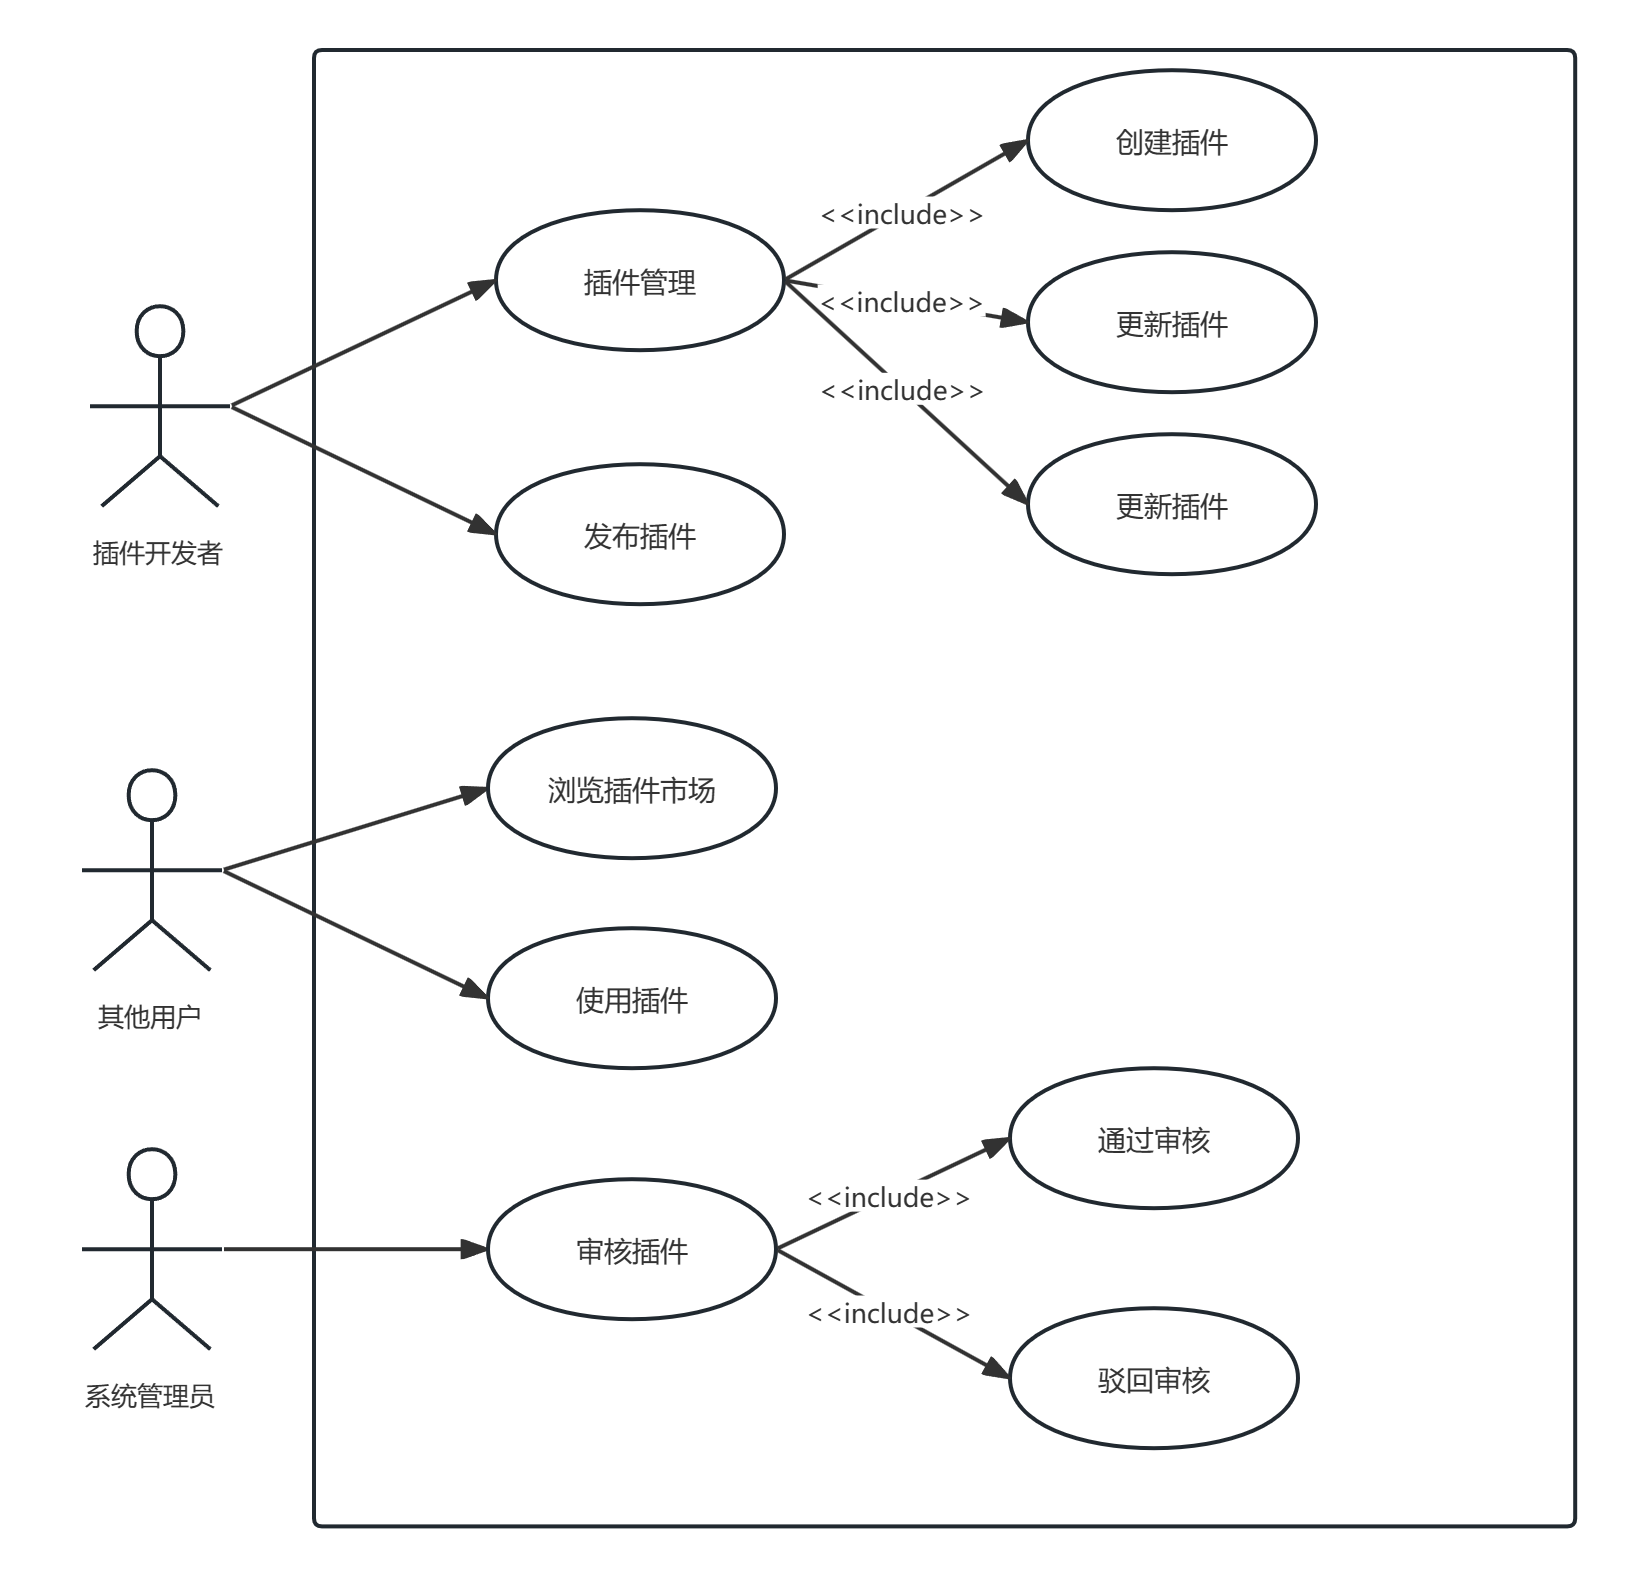
\includegraphics[width=0.7\textwidth]{插件市场用例图.png}
  \caption{插件市场用例图}
  \label{fig:插件市场用例图}
\end{figure}

\subsection{状态流转需求}
在流水线的执行过程中,流水线中的每个子概念都在不同的状态间流转,通常来说应有如下状态:
就绪中(Pending)、执行中(Running)、执行成功(Success)、执行失败(Failed)、被跳过(Skipped)、被取消(Canceled)。

CI/CD调度系统需要保障流水线作业能够进行正确的状态流转,以保证用户能够正确、及时地得知流水线的执行情况。
同时,状态的正确流转也是流水线能按照正确逻辑链路执行的保证,系统需要结合当前流水线内各个子概念的状态,结合用户的人为操作,来判断流水线接下来的状态。

\subsection{自动触发需求}
自动化是CI/CD流水线提高软件团队研发效能的保证。通常来说,用户会希望某个指定仓库的代码出现变更的时候,CI/CD系统中的流水线便能自动触发。
系统能够某种感知或监听

\subsection{流水线作业合理调度需求}
\label{subsec:流水线作业合理调度需求}

作业是流水线执行器中执行的最小单位,CI/CD调度器作为流水线配置与作业实际执行环境的中间环节,需要从作业排队、一致性分发、统一调度等方面保证作业的合理调度。

首先,系统需要保证作业的执行顺序与其被调度的顺序一致,即先来先执行。其次,当相当数量的作业被调度,超过了执行器的承载能力时,系统应能保证作业的阻塞等待,当前执行的作业结束执行后,再执行阻塞中的作业。
以上两点需求业内往往借助开源的消息队列服务实现,如RocketMQ等,借助消息队列先进先出和持久化的特性,保证了作业的调度顺序和阻塞等待。

然后,系统需要完成流水线作业的分配任务,将作业能够合理的分配给不同的作业执行模块。
当调度器判断应该调度某个作业时,CI/CD调度器将根据流水线配置时用户预填写的内容封装作业信息,再交付给执行器执行任务。
这一特性往往通过消息队列中消息的Tag和Title概念来实现对作业的精确分配。
同时,系统需要能够保证一个作业只能被一个执行器所执行,不能被多个执行器重复执行。


\section{非功能性需求}

除功能性需求外,系统需要满足以下非功能需求:

\subsubsection{高性能}
本系统致力于提升效能,提高用户的研发效率,需要保证优秀的性能和较短的响应时间。
当用户进行流水线管理时,对流水线配置的增删改查应在1s内完成;
当用户人为干预流水线时,系统应在2s内给予用户反馈;
当流水线中阶段、作业或者任务的状态发生改变时,应在5s内对用户进行展示。

\subsubsection{高稳定性}
CI/CD流水线系统的可靠性和稳定性尤为重要,一旦系统发生故障则直接影响整个企业的开发人员、测试人员和运维人员,阻塞代码合并、业务提测、系统发布等流程。
本系统可以借助以Kubernetes为代表的容器编排系统,实现横向扩展和故障转移的能力,以保证系统在使用高峰期时的稳定性。

\subsubsection{高可用性}
CI/CD在当今的软件开发流程中是不可缺少的一环,系统应尽量保证7×24小时的服务提供。
依据业界常用指标,本系统需要至少达到99.99\%的可用性。
换算成服务时间则根据公式:服务可用率=成功调用数/总调用数,系统每一年的时间内,无法提供服务的总时间不能超过52分钟。

\subsubsection{高易用性}
本系统应提供友好的交互逻辑,让缺乏相关知识背景的用户能够快速找到流水线的编辑与配置方式;
同时,由于CI/CD流水线通常有着复杂的层级与结构,系统应提供所见即所得的流水线拓扑结构界面,以便用户查看和调整;
最后,流水线的执行过程中应提供入口,将各个作业的运行日志可视化地展示给用户,方便用户时刻监控流水线作业的执行情况。

\subsubsection{高安全性}
流水线一旦执行,可能会对其对应的系统产生影响,如发布新版本、发送通知等等。
为避免产生不期望的后果,系统应对流水线的触发以及各种操作进行严格的权限控制。
比如对某一条流水线的任何人为干预操作都应该由只能由流水线的归属人执行,其他人操作则提示无权限。
